\section{Gerador de analisadores léxicos}

\begin{frame}[fragile]{Flex}

    \begin{itemize}
        \item Flex (\textit{Fast Lexical Analyzer Generator}) é um programa para a geração de analisadores léxicos
       %\pause

        \item Ele foi escrito em linguagem C por Vern Paxson por volta de 1987
       %\pause

        \item Ele pode ser usado em conjunto com um gerador de analisadores sintáticos (por exemplo, o Yacc e o GNU Bison)
       %\pause

        \item Flex é mais flexível e gera códigos mais rápidos que o Lex, outro programa gerador de analisadores léxicos
       %\pause

        \item Ele pode ser instalado, em distribuições Linux baseadas no Debian, por meio do comando
            \inputsyntax{sh}{codes/install.sh}
    \end{itemize}

\end{frame}

\begin{frame}[fragile]{Fluxo de uso do Flex para geração de analisadores léxicos}

    \begin{figure}
        \centering 

        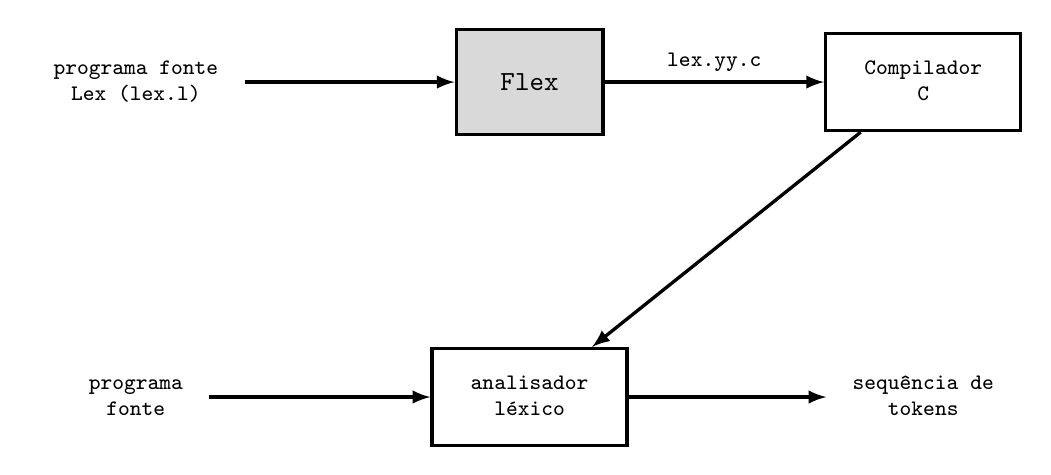
\begin{tikzpicture}
            \node (A) at (0, 6) {\footnotesize \texttt{\begin{tabular}{c}programa fonte\\ Lex (lex.l)\end{tabular}} };
            \node[draw,very thick,inner sep=16pt,fill=gray!30] (B) at (5, 6) {\texttt{Flex}};
            \node[draw,very thick,inner sep=8pt] (C) at (10, 6) {\footnotesize \texttt{\begin{tabular}{c}Compilador\\ C\end{tabular}} };
            \node[draw,very thick,inner sep=8pt] (D) at (5, 2) {\footnotesize \texttt{\begin{tabular}{c}analisador \\ léxico\end{tabular}} };
            \node (E) at (10, 2) {\footnotesize \texttt{\begin{tabular}{c}sequência de\\ tokens\end{tabular}} };
            \node (F) at (0, 2) {\footnotesize \texttt{\begin{tabular}{c}programa \\ fonte\end{tabular}} };

            \draw[very thick,-latex] (A) to (B);
            \draw[very thick,-latex] (B) to node[above] { \footnotesize \texttt{lex.yy.c} } (C);
            \draw[very thick,-latex] (C) to (D);
            \draw[very thick,-latex] (D) to (E);
            \draw[very thick,-latex] (F) to (D);
        \end{tikzpicture}
    \end{figure}


\end{frame}

\begin{frame}[fragile]{Programas Lex}

    \begin{itemize}
        \item Programas Lex são salvos em arquivos com extensão \texttt{.l} (ou \texttt{.lex})
       %\pause

        \item Este programas exportam uma função chamada \code{c}{yylex()} que, ao ser chamada, extraí o próximo token do programa fonte
       %\pause

        \item O código gerado (arquivo \texttt{lex.yy.c}) pode ser usado para gerar um executável independente, ou pode ser compilado como código objeto e ser
            integrado ao analisador sintático
       %\pause

        \item Os programas Lex são dividos em três partes: a seção de definições, a seção de regras e a seção de códigos de usuário
       %\pause

        \item A vantagem do uso de programas Lex é que eles permitem a especificação dos tokens por meio de expressões regulares, e a implementação dos
            diagramas de transição é feita automaticamente pelo Flex
    \end{itemize}

\end{frame}

\begin{frame}[fragile]{Seção de definições}

    \begin{itemize}
        \item Nesta seção são declaradas variáveis, constantes e definições regulares
       %\pause

        \item As declarações desta seção deve ser delimitado pelas sequências de caracteres \verb|"%{"| 
            e \verb|"%}"|
       %\pause

        \item O conteúdo desta seção é copiado diretamente para o arquivo \texttt{lex.yy.c}
       %\pause

        \item As definições regulares devem ser declaradas após as definições, na forma
            \inputsyntax{sh}{codes/dec.syntax}
       %\pause

        \item Uma vez definido um nome, ele pode ser usado nas definições regulares subsequentes, desde que esteja delimitado por chaves
    \end{itemize}

\end{frame}

\begin{frame}[fragile]{Exemplo de seção de declarações}
    \inputsnippet{cpp}{1}{10}{codes/lex.l}
    \inputsnippet{bash}{12}{17}{codes/lex.l}
\end{frame}

\begin{frame}[fragile]{Seção de regras}

    \begin{itemize}
        \item Esta seção contém uma série de regras, uma por linha, na forma
            \inputsyntax{sh}{codes/dec2.syntax}
       %\pause

        \item O padrão não deve estar indentado e deve estar na mesma linha da ação
       %\pause

        \item O padrão pode conter algum nome presente nas declarações regulares
       %\pause

        \item Neste caso, o nome deve ser delimitado por chaves
       %\pause

        \item Esta seção é delimitada pela sequência de caracteres \verb|%%|
    \end{itemize}

\end{frame}

\begin{frame}[fragile]{Exemplo de seção de declarações}
    \inputsnippet{cpp}{19}{35}{codes/lex.l}
\end{frame}

\begin{frame}[fragile]{Seção de código de usuário}

    \begin{itemize}
        \item Esta seção também é copiada diretamente para o arquivo \texttt{lex.yy.c}
       %\pause

        \item Uma outra alternativa é definir estes códigos em arquivos separados e depois carregar este código na compilação do analisador léxico
       %\pause

        \inputsnippet{cpp}{37}{49}{codes/lex.l}
    \end{itemize}

\end{frame}

\begin{frame}[fragile]{Exemplo de função {\tt main()} para um analisador léxico independente}

    \inputsnippet{cpp}{51}{70}{codes/lex.l}

\end{frame}
